\chapter{WordPress}
\label{chp:wp}
L'analisi dei requisiti ha evidenziato la necessità di un sito web in cui esporre e descrivere al cliente i servizi offerti, aggiornato e popolato da un componente del team di {\fem} non per forza munito di conoscenze e capacità tecniche informatiche; la scelta é ricaduta su \emph{\wp}.

{\wp} è una piattaforma software di Content Management System (CMS), ovvero un programma installato sul server che consente la creazione, gestione, distribuzione e manutenzione di un sito Internet \cite{wordpress}. È un progetto open-source creato da Matt Mullenweg e distribuito con la licenza GNU General Public License, sviluppato in PHP con appoggio a MySQL come gestore di database.

\section{Caratteristiche di {\wp}}
{\wp} permette il download gratuito dal sito \url{www.wordpress.org} di tutti i suoi componenti base necessari per l'installazione sulla propria macchina. Esiste anche un servizio a pagamento, con prezzo variabile in base alle richieste, chiamato \emph{WordPress.com}, che permette di costruire rapidamente il proprio sito web o blog basato su {\wp} senza la necessità di possedere un server o competenze tecniche specifiche.

{\wp} permette di estendere le proprie funzionalità con l'ausilio di opportuni plugin, ovvero moduli che aggiungono caratteristiche ed elementi all'applicativo; i plugin possono essere gratuiti o a pagamento e possono fare di tutto, dal potenziare l'editor testuale integrato, all'inserire slideshow o gallerie di immagini nelle pagine, e molto altro ancora. Analogamente ai plugin si possono trovare anche temi, cioè estensioni che permettono di personalizzare l'aspetto del sito modificando sfondi, impaginazione, font, etc.

\section{{\wp} per il Portale Avifauna}
Per realizzare il \emph{Portale della Diagnostica Molecolare dedicato all'Avifauna} é stato installato e configurato {\wp} all'indirizzo del sottominio scelto 

\texttt{www.avifauna.fem2ambiente.com}

Sul sito \url{www.wordpress.org} è possibile scaricare l'ultima versione di {\wp} (ad oggi, Ottobre 2015, è la numero 4.3.1), una volta effettuato il download è necessario seguire le istruzioni fornite nel file \texttt{readme.html} \cite{installing_wordpress}, in particolare:
\begin{itemize}
 \item creare un database dedicato utilizzando MySQL;
 \item eseguire le opportune modifiche al file \texttt{wp-config.php} in un editor di testo;
 \item attivare una connessione sicura con il server e caricare tutti i file di installazione di {\wp} nella cartella scelta (in questo caso \texttt{/home});
 \item configurare in modo appropriato seguendo le istruzioni fornite nella pagina

 \texttt{http://avifauna.fem2mabiente.com/home/wp-admin/install.php}
\end{itemize}

Una volta terminata l'installazione sono stati installati alcuni plugin, temi ed estensioni considerati necessari.

La scelta del tema è ricaduta su \emph{Everest} di YOOtheme (Versione: 1.0.11). 

YOOtheme è una azienda tedesca che produce componenti per CMS \cite{yootheme}; i loro prodotti più importanti, oltre a una ventina di temi e template rispettivamente per {\wp} e Joomla!, sono \emph{Wrap Framework} \cite{wrap} e \emph{Uikit} \cite{uikit}, due architetture software di supporto per la creazione e personalizzazione dei componenti aggiuntivi ai più famosi CMS.

Il tema Everest è stato costruito utilizzando Wrap Framework e mette a disposizione dell'utilizzatore sette stili di layout differenti, personalizzazioni nella costruzione del layout sfruttando tutte le potenzialità di {\wp} e un pacchetto di plugin chiamato \emph{Widgetkit} per l'inserimento rapido di Slideshow, gallierie di immagini, mappe. Per tutte queste caratteristiche è stato scelto, acquistato ed installato come tema per il sito.

Per ricoprire tutti i bisogni organizzativi di un sito commerciale come il Portale Avifauna è stato necessario installare anche \emph{Polylang} \cite{polylang} per il supporto multilingue al sito e \emph{My Calendar} \cite{mycalendar} per la gestione degli eventi.

Dopo aver creato e popolato il sito con i contenuti, il risultato ottenuto è visibile nell'immagine~\ref{fig:homepage} e al seguente indirizzo \url{www.avifauna.fem2mabiente.com/home}.

\begin{figure}
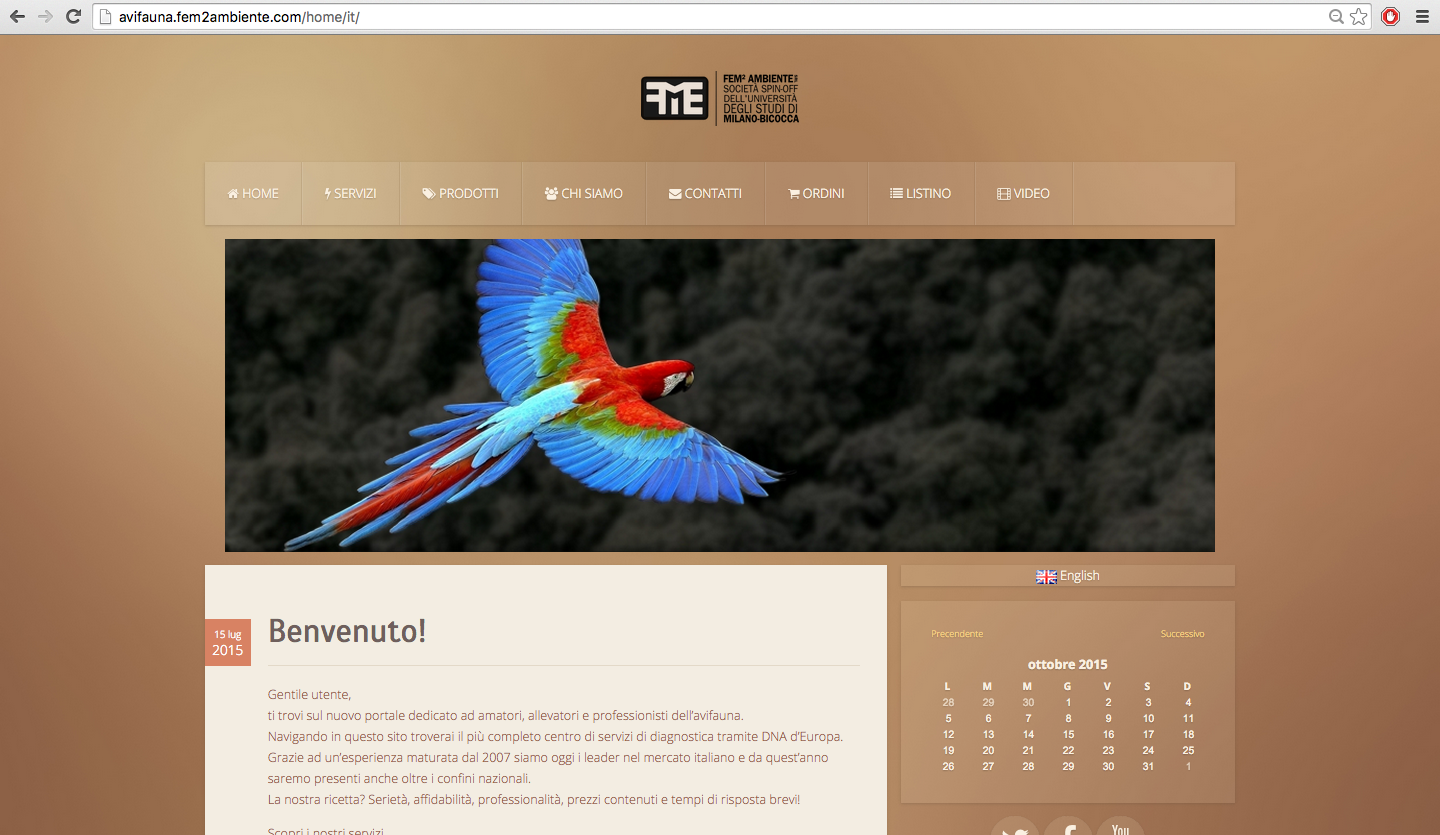
\includegraphics[width=1\textwidth]{images/homepage-wp} 
\caption{homepage del Portale per la Diagnostica Molecolare Avifauna}
\label{fig:homepage}
\end{figure}

Cliccando sul tasto \textsf{Ordini} (come in figura~\ref{fig:homepage-ordini}) si può accedere alla piattaforma personalizzata descritta nei seguenti capitoli.

\begin{figure}
 \centering
 
\includegraphics[width=0.3\textwidth]{images/homepage-wp-ordini} 
 \caption{tasto per accedere alla sezione ordini}
 \label{fig:homepage-ordini}
\end{figure}